\part{Algorithms}
\frame{\partpage}

\begin{frame}{What is an algorithm?}
	\pause\begin{center}
		A \textbf{sequence of instructions} which can be followed \textbf{step by step}
		to perform a \textbf{(computational) task}.
	\end{center}
\end{frame}

\begin{frame}{Algorithms historically}
	\begin{itemize}
		\pause\item Named after Muhammad ibn Musa al-Khwarizmi (c.\ 780--850), Persian mathematician
		\pause\item Used in mathematics to describe steps for calculations
            \begin{itemize}
                \pause\item E.g. Euclid's algorithm for finding the greatest common divisor of two numbers
            \end{itemize}
        \pause\item Computers developed as machines for carrying out mathematical algorithms
	\end{itemize}
\end{frame}

\begin{frame}{Programs vs algorithms}
	\begin{itemize}
		\pause\item A program is \textbf{specific} to a particular programming language and/or machine
		\pause\item An algorithm is \textbf{general}
		\pause\item An algorithm must be \textbf{implemented} as a program before a computer can run it
		\pause\item An algorithm generally performs \textbf{one task}, whereas a program may perform \textbf{many}
		\begin{itemize}
			\pause\item E.g.\ Microsoft Word is not an algorithm, but it implements many algorithms
			\pause\item E.g.\ it implements an algorithm for determining where to break a line of text,
				how much space to add to centre a line, etc.
		\end{itemize}
	\end{itemize}
\end{frame}

\begin{frame}{Algorithms outside computing}
	\begin{center}
		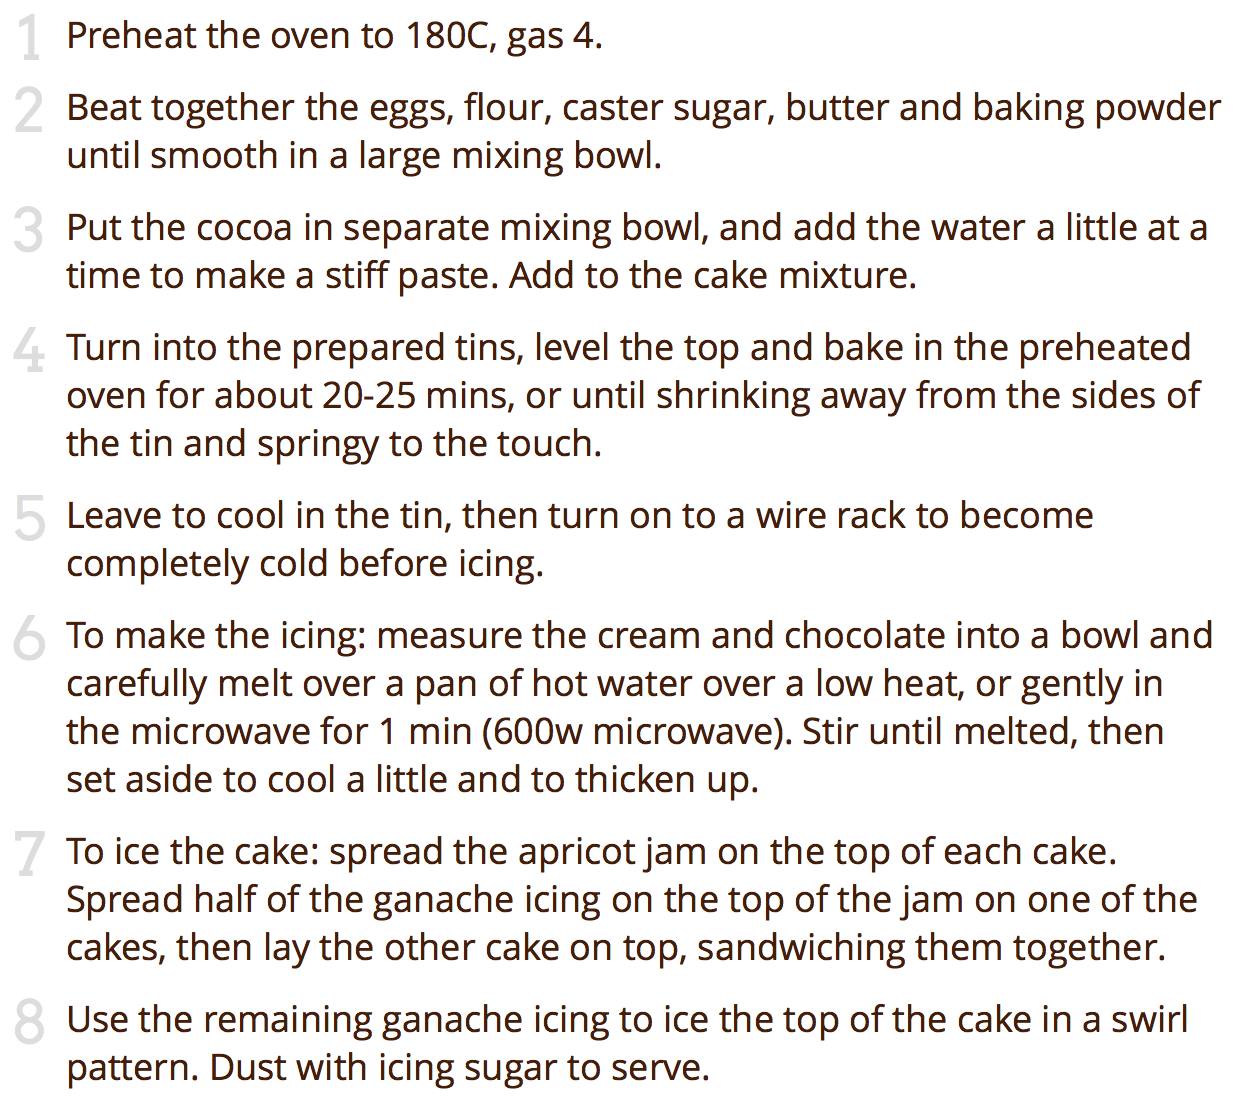
\includegraphics[height=0.8\textheight]{cake_recipe}
	\end{center}
\end{frame}

\begin{frame}{Algorithms outside computing}
	\begin{center}
		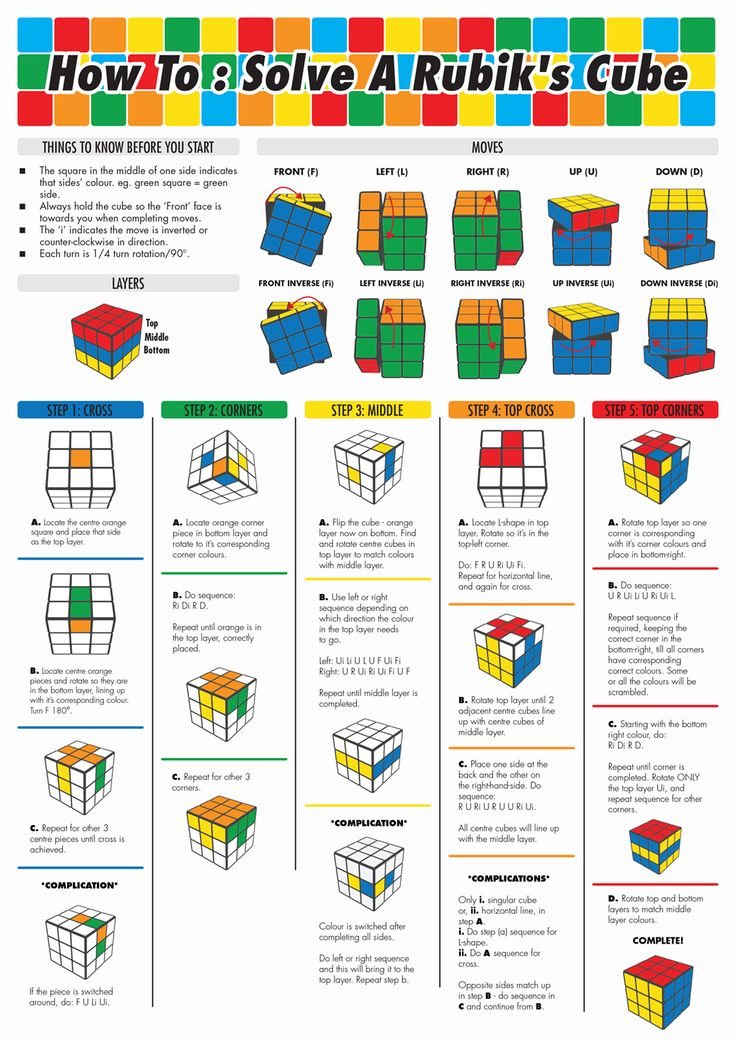
\includegraphics[height=0.8\textheight]{rubik_algorithm}
	\end{center}
\end{frame}

\begin{frame}{Why algorithms?}
	\begin{itemize}
		\pause\item Allow for common computations to have \textbf{common solutions}
		\pause\item \textbf{Algorithm strategies} give widely applicable approaches for solving problems
		\pause\item Can \textbf{prove} mathematically that an algorithm does what it is supposed to
		\pause\item Can reason about the \textbf{complexity} (time, space etc) of an algorithm
		    --- and place \textbf{lower bounds} on the best possible algorithm
		\pause\item \textbf{Computability} theory lets us reason about what computations are and are not possible
	\end{itemize}
\end{frame}

